%%!TEX encoding = UTF-8 Unicode
\documentclass[11pt, letterpaper, onecolumn, english, notitlepage]{book}

\usepackage[left=1.5in, right=1.5in, top=1.5in, bottom=1.5in]{geometry}
\usepackage[cc]{titlepic}
\usepackage{amsmath, graphicx, hyperref, subcaption, amssymb, amsthm}
\usepackage[none]{hyphenat}
\usepackage{geometry}
\usepackage{xspace}
\usepackage{epstopdf}
%\usepackage[frenchb]{babel}
\usepackage[utf8]{inputenc}
\usepackage[T1]{fontenc}
\DeclareGraphicsRule{.tif}{png}{.png}{`convert #1 `dirname #1`/`basename #1 .tif`.png}

\linespread{1}
\hypersetup{colorlinks=false, linkbordercolor={1 1 1}, citebordercolor={1 1 1}, urlbordercolor={1 1 1}}

\newcommand{\mref}[2]{\hyperref[#1]{#2\ref*{#1}}}
\newcommand{\emref}[2]{\hyperref[#1]{#2(\ref*{#1})}}
%\newtheorem{Lemma}{Lemma}
%\newtheorem*{solution}{Solution}

\begin{document}

    \begin{titlepage}
        \begin{center}
            \title{Documentation of the MATLAB and \LaTeX{} framework (Faryadell)}
            \author{
                \textbf{Abolfazl Delavar}\\
                \\
                Version \textbf{1.0.0}\\
                \\
                Control Engineering \& Computational Neuroscience\\
                \href{http://abolfazldelavar.com}{http://abolfazldelavar.com}\\
                \href{mailto:faryadell@gmail.com}{faryadell@gmail.com}
            }
            \date{\today}
            
\includegraphics[width=0.4\linewidth,trim=2 2 2 2,clip=true]{img/framework.png}
        \end{center}

    \end{titlepage}

    \maketitle

    \newpage

    \tableofcontents

    
    \vspace{2.5cm}
    \chapter{Introduction} {
        \newpage
        \paragraph{a)} {
We have
    \begin{equation*}
        s(i)=\frac{t^2(i)}{2}.g
    \end{equation*}
such that
    \begin{equation*}
        \theta = g \quad \& \quad \varphi^T(i)=\frac{t^2(i)}{2}
    \end{equation*}
Also the Least Squares problem is
    \begin{equation} \label{eq.2}
        \hat{\theta}(i) = \left(\sum_{j=1}^{i}\varphi(j)\varphi^T(j)\right)^{-1}\left(\sum_{j=1}^{i}\varphi(j)y(j)\right).
    \end{equation}
for find $g$, assume that $s(i)=[0,5,19.5,44]$ and $t(i)=[0,1,2,3]$ for $i=[1,2,3,4]$. therefor
\begin{align}
    P(4) = \left(\sum_{i=1}^{4}\left(\frac{t^2(i)}{2}\right)^2\right)^{-1} &= 0.0408\nonumber\\
    g_1=\hat{\theta}_1(i=4)= P(4)\left(\sum_{j=1}^{4}\left(\frac{t^2(j)}{2}\right)s(j)\right) &= 9.7755.
\end{align}
}
\paragraph{b)} {
    Recurcive Least Squares for calculate one forward step with new point $s(5)=78.5$ and $t(5)=4$:
    \begin{align}
        P(5) = \left(P^{-1}(4) + \varphi(5)\varphi^T(5)\right)^{-1} &= 0.0156\nonumber\\
        g_2 = \hat{\theta}_2(5) = \hat{\theta}_1(4) + P(5)\varphi(5)\left(s(5) - \varphi^T(5)\hat{\theta}_1(4)\right) &= 9.8125.
    \end{align}
}
    }

    \newpage
    \chapter{Object Oriented Programming (OOP)} {
        \newpage
        \section{Introducing OPP}
    \subsection{Class}

    \subsection{Object}

\section{Inheritence}

\section{Examples}

In \emref{eq.2}{Eq } if 
\begin{equation}
    y(t)=\phi^T(t)\theta(t) + e(t)
\end{equation}
such that, $e(t)$ is a white noise with zero mean and variance $\sigma^2$, then
\begin{align*}
    \hat{\theta}(i) = \theta + \left(\sum_{j=1}^{i}\varphi(j)\varphi^T(j)\right)^{-1}\left(\sum_{j=1}^{i}\varphi(j)e(j)\right).
\end{align*}
therefore, 
\begin{equation}
    E\{\hat{\theta}\}=\theta .
\end{equation}
On the other hand we know that
\begin{align}
    \mathrm{var}(\hat{\theta}) = E\{\hat{\theta}^2\} - E^2\{\hat{\theta}\}.
\end{align}
\begin{proof}
We expand the given equation on both side:
\begin{align}
    E\{(\hat{\theta}-\theta)^2\} &= E\{\hat{\theta}^2 + \theta^2 - 2\theta\hat{\theta}\}\\
    &= E\{\hat{\theta}^2\} + E\{\theta^2\} - 2E\{\theta\hat{\theta}\} \nonumber\\
    &= \theta^2 + E\{\hat{\theta}^2\} - 2\theta E\{\hat{\theta}\}.\nonumber\\
    &\nonumber\\
    bias^2 + var &= (\theta - E\{\hat{\theta}\})^2 + E\{\hat{\theta}^2\} - E^2\{\hat{\theta}\}\\
    &= \theta^2 + E\{\hat{\theta}^2\} - 2\theta E\{\hat{\theta}\}.\nonumber
\end{align}
The both side of equation are equal, so the proof is complete.
\end{proof}
    }

    \newpage
    \chapter{Fundamental of Dynamical Systems} {
        \newpage
        \section{Ordinary Differential Equations (ODEs)} {
    \subsection{Linear Time Invariant (LTI)} {
        \subsubsection*{LTI systems without input delay} {
            
        }
        \subsubsection*{LTI systems with delayed inputs} {

        }

    }
    \subsection{Nonlinear ODEs without input delay} {

    }
    \subsection{Nonlinear ODEs with delayed inputs} {

    }
}
\section{Partial Differential Equations (PDEs)} {

}
\section{Examples} {

}
For estimation the parameters, using the `ARX' command in MATLAB, we achieve the \mref{tab.est}{Table }.
Model 4 is better than other models, because MSE is small and Fit percent is bigger than others.
But why model 5 is not good? It is not a good model because $a_2\simeq 0$ and there is not much difference between model 4 and model 5.
therefore model 4 with fewer poles is a good select for Representation system.
\begin{table}[h!]
    \begin{center}
        \caption{Estimated Parameters with LS method}
        \label{tab.est}
        \begin{tabular}{c|c|c|c|c|c|c}
            Model &  $a_1$ & $a_2$ & $b_1$ & $b_2$ & MSE & Fit(\%)\\
            \hline
            1 & - & - & $0.9078$ & $-0.9212$ & $0.3727$ & $58.87$ \\
            2 & $-0.7390$ & - & $0.8832$ & - & $0.1705$ & $72.18$\\
            3 & $-0.9856$ & $-0.3485$ & $0.9315$ & - & $0.04384$ & $85.89$\\
            4 & $-0.5229$ & - & $0.9033$ & $-0.4809$ & $0.003321$ & $96.12$\\
            5 & $-0.525$ & $-0.001746$ & $0.9035$ & $-0.479$ & $0.00332$ & $96.12$\\
        \end{tabular}
    \end{center}
\end{table}
    }

    \newpage
    \chapter{MATLAB framework} {
        \newpage
        \section{Introduction of the models structure} {
	\paragraph{} {
		The provided framework is shared to help scientists working on system engineering, control, computational neuroscience, robotic, etc.
		This package contains several simple files that connect to each other like diagram illustrated in \mref{fig:1}{Fig. }. As it is clear from \mref{fig:1}{Fig. }, '\texttt{main.m}' is the file which must be called to run the simulation.
		Note that running other files is not recommended, although it can be usefull in some situations. 
		There are 5 called functions in the '\texttt{main.m}' file which will be elaborated in the following.
	}
	\begin{figure}[b!]
		\centering{
			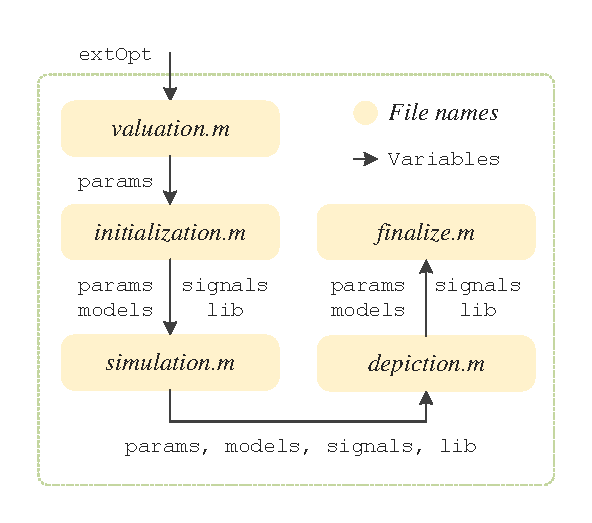
\includegraphics[width=0.6\linewidth,page=1,trim=4 4 4 4,clip=true]{img/pdf/mainDiagram.pdf}
			\caption{The internal blocks of '\texttt{main.m}' file.}
			\label{fig:1}
		}
	\end{figure}
}

\section{Framework files and directories} {
	\subsection{Basic files} {
		\paragraph{} {
			The group of all files exist in the main root is named basic files, such as '\texttt{main.m}', '\texttt{simulation.m}', and so forth.
		}

		\subsubsection{'main.m'} {
			If you are a person who want to run the simulation once, it just need to write '\texttt{main}' in the command window.
			However, if the project is developed to simulate several times, you should make a structure variable of necessary parameters, e.g. '\texttt{extOpt}', and insert it into the '\texttt{valuation(extOpt)}' function existed in the main file.
			After that, by calling '\texttt{main.m}' using the expression '\texttt{run main.m}', you can have a control to your main file for multi-run simulations.
			This command can be used in a '\texttt{for}' loop in your mother file to run the simulation, get and save the results, repeatedly.
			Note that, it might be helpful if '\texttt{close all; clear; clc;}' expression in '\texttt{main.m}' is removed, but it can dependent on your project purposes.
		}

		\subsubsection{'valuation.m'} {
			\paragraph{} {
				The first function named '\texttt{valuation.m}' is considered to collect all static variables such as simulation time and step-time.
				You can define your constant variables in this function in a structure variable named '\texttt{params}'.
				For example, to set a constant value, which is represents $\pi$, you have to write '\texttt{params.pi = 3.14;}' into the function '\texttt{valuable.m}'.
				\mref{fig:2}{Figure } is an image of this function.
			}
			\begin{figure}[tbp]
				\centering{
					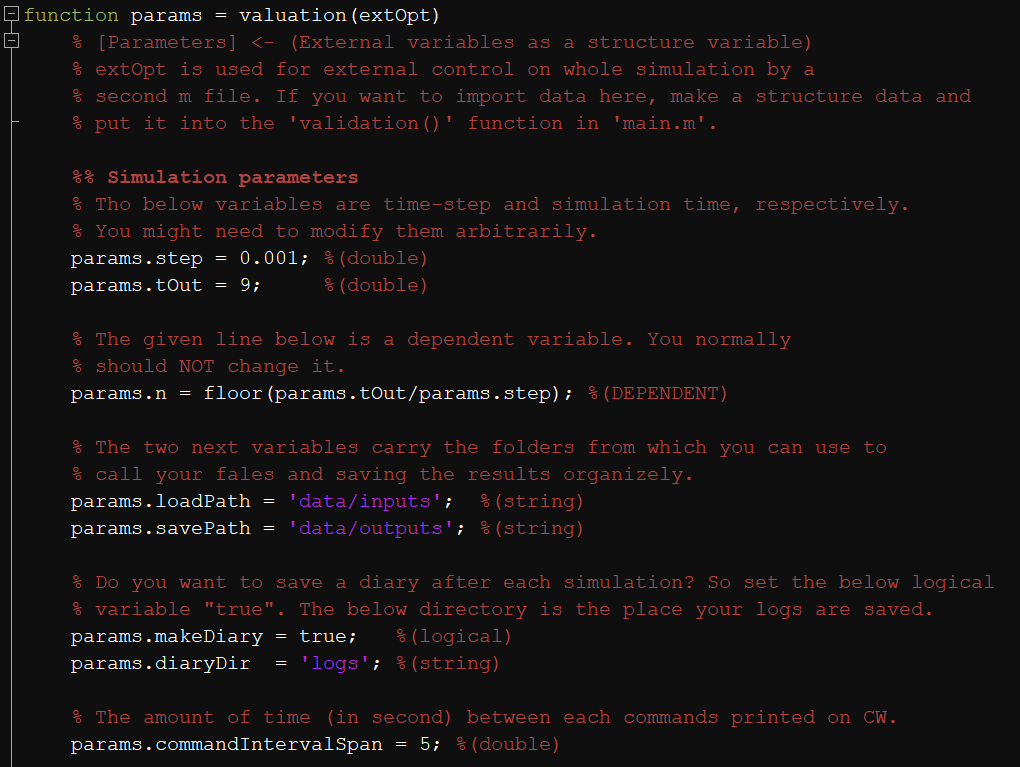
\includegraphics[width=0.95\linewidth,page=1,trim=0 0 0 0,clip=true]{img/matlab/valuation.png}
					\caption{The content inside the '\texttt{valuation.m}'.}
					\label{fig:2}
				}
			\end{figure}
		}

		\subsubsection{'initialization.m'} {
			\paragraph{} {
				The second file, which is considered as a part of initial tasks before the main simulation, can be undoubtedly mentioned as '\texttt{initialization.m}'.
				The same as '\texttt{valuation.m}', it carries kinds of data that is always used in the whole project, while it is not important to have constant values.
				In other words, here, we usually define vectors and signals in a structure variable named '\texttt{signals}'.
				Also, all synamic systems, filters, estimators, trackers , etc, must be define in this file in a uniqe variable which is '\texttt{models}'.
				Furthermore, in some projects, several fixed parameters must be set after some initializations.
				To satisfy this, the parameter structure '\texttt{params}' can be change at the end of '\texttt{initialization.m}' file.
				In addition, some useful libraries (Groups of functions) are added in this file which will be explained later.
				To sum up, This function receives '\texttt{params}' as its input variables and after an initial process, four structure variables named '\texttt{params}', '\texttt{models}', '\texttt{signals}', and '\texttt{lib}' are sent to the out. \mref{fig:3}{Figure }, illustrates a view of this function.
			}
			\begin{figure}[tbp]
				\centering{
					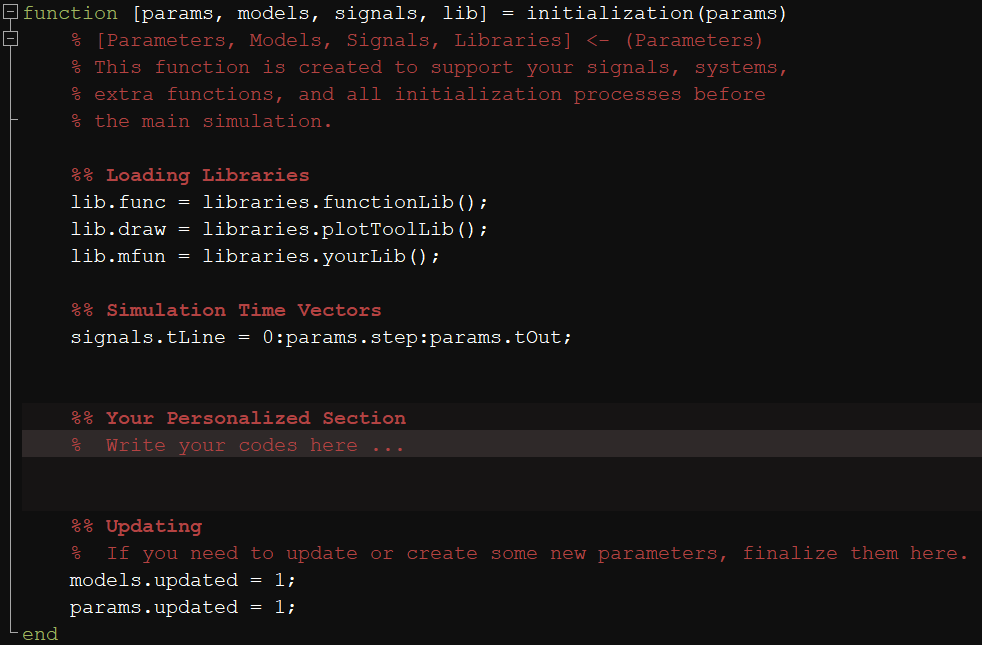
\includegraphics[width=0.90\linewidth,page=1,trim=0 0 0 0,clip=true]{img/matlab/initialization.png}
					\caption{The content inside the '\texttt{initialization.m}'.}
					\label{fig:3}
				}
			\end{figure}
		}

		\subsubsection{'simulation.m'} {
			\paragraph{} {
				It should be mentioned that this file is the most important file in which you have to plan and control your main idea.
				In other words, the main loop of your simulation has been written in '\texttt{simulation.m}'.
				All variables that are resulted from '\texttt{initialization.m} directly came to this file and all of them finally are led to the output.
				The first part of this file is just before the loop which you can prepare your temporary initial variables that might be used in the loop.
				To do this, write your codes at the end of '\texttt{Initial options}' part, just before the '\texttt{for}' loop.
				The counter variable of this loop, which is '\texttt{k}', is a '\texttt{double}' variable that starts from zero and is increased up to '\texttt{params.n}', which is the number of simulation samples.
				It is clear that this variable depends on the simulation time and step-time which is set in '\texttt{valuable.m}'.
				At the begining of the loop, there is an order that is put to make a report of loop condition.
				To be exact, it prints a line into the command windows that contains the current sample '\texttt{k}', the number of all samples, the progress percentage, and expecting time to the end of the simulation.
				This report is normally printed each 5 seconds and can be helpful to know how much of the process has done and how much we must be waiting to be completed.
				The amount of this span is under your control in variable '\texttt{commandIntervalSpan}' that is defined in '\texttt{valuation.m}' function.
				After the '\texttt{for}' loop, we can see a part named '\texttt{Finalize options}', which are utilized to report total simulation time, although you can exploit that for your purposes.
				A case of this function is demonstrated in \mref{fig:4}{Fig. }, and \mref{fig:5}{Fig. } shows the final situation of command window after ending a program.
			}
			\begin{figure}[tbp]
				\centering{
					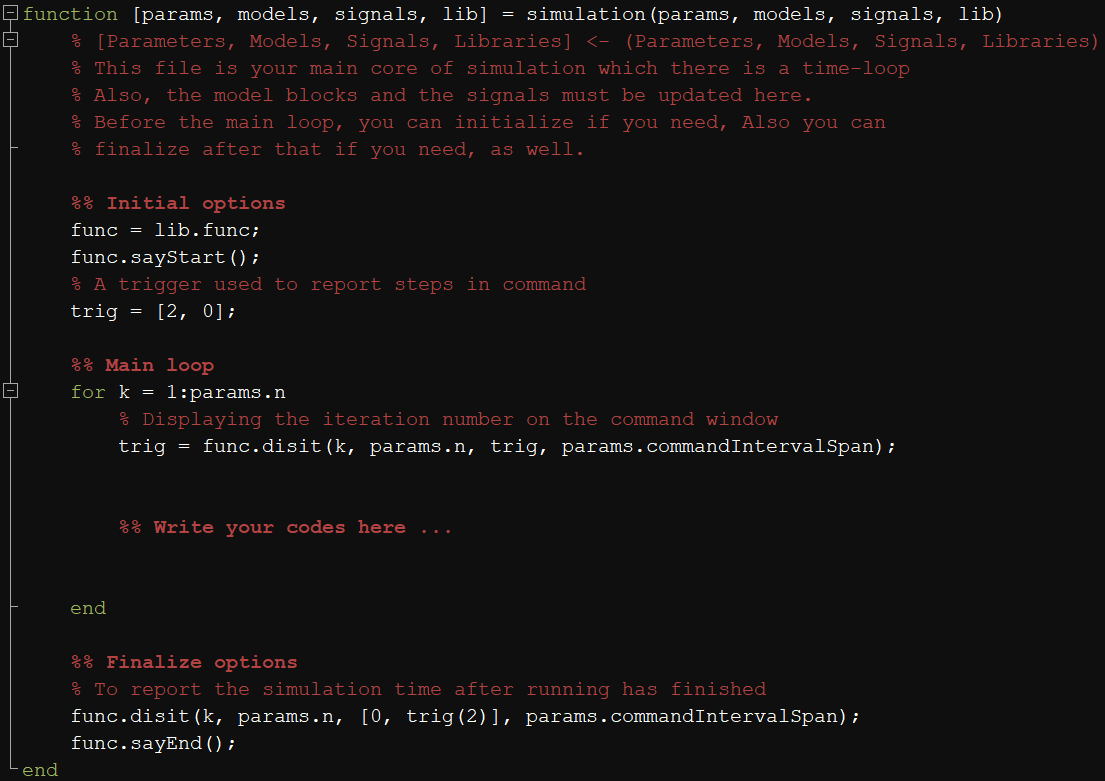
\includegraphics[width=0.80\linewidth,page=1,trim=0 0 0 0,clip=true]{img/matlab/simulation.png}
					\caption{The content inside the '\texttt{simulation.m}'.}
					\label{fig:4}
				}
			\end{figure}
			\begin{figure}[tbp]
				\centering{
					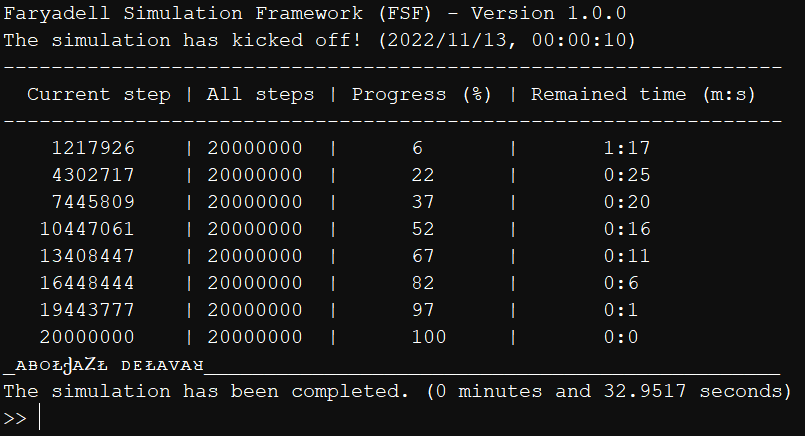
\includegraphics[width=0.80\linewidth,page=1,trim=0 0 0 0,clip=true]{img/matlab/command.png}
					\caption{Outputs of a project that printed in the command window. As it is distinct, the simulation ran about 50 seconds.}
					\label{fig:5}
				}
			\end{figure}
		}

		\subsubsection{'depiction.m'} {
			\paragraph{} {
				Do you need to make your data graphical? If you do, here is all you need to plot and depict your novels.
				As it can be clearly seen that in \mref{fig:6}{Fig. }, which is a shot of this function, all quadruple variables are ready to be used here and by thanks of its outputs, it is also possible to modify them, although it is not really common to make any changes after the simulation stage.
				In addition, one more variable defined at the end of input arguments whose name is '\texttt{plotOrNot}'.
				This is beneficial for you, in case of ignoring the depiction section.
				To do this, it must be set '\texttt{false}' in the '\texttt{main.m}' file.
				Note that the default value of this logical variable is '\texttt{true}' which means the illustrator section is enabled.
				As the same as before, this function is splitted into three parts which named '\texttt{Initialize}', '\texttt{Main part}', and '\texttt{Finalize}', respectively.
				The first and last part are used to define initial variables and finalize the plot section.
				The main part of the file that can be mentioned is the middle part.
				All MATLAB functions related to graphic, and also a practical library called '\texttt{plt}' are ready to be exploited there.
				Finally, there is nothing more especial here, and the most effective parts of this framework which concentrates on graphics will be elaborated in libraries and observer parts.
			}
			\begin{figure}[tbp]
				\centering{
					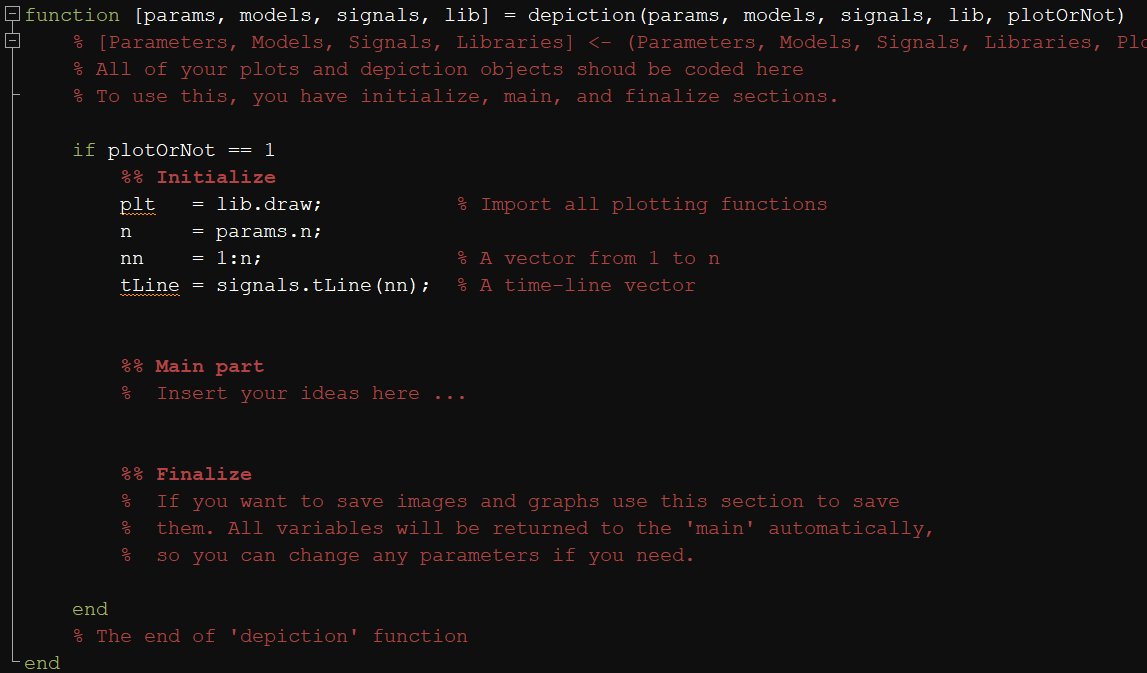
\includegraphics[width=1\linewidth,page=1,trim=0 0 0 0,clip=true]{img/matlab/depiction.png}
					\caption{A shot of '\texttt{depiction.m}' file.}
					\label{fig:6}
				}
			\end{figure}
		}

		\subsubsection{'finalize.m'} {
			\paragraph{} {
				The last file of the main root is '\texttt{finalize.m}' to be utilized for saving obtained data and report some pieces of them on the command window.
				This function is almost empty at the first, except the order which turn the started diary off, but you can call all variables which is available into that to code your remained ideas. \mref{fig:7}{Figure } is a simple shot of '\texttt{finalize.m}' function.
			}
			\begin{figure}[tbp]
				\centering{
					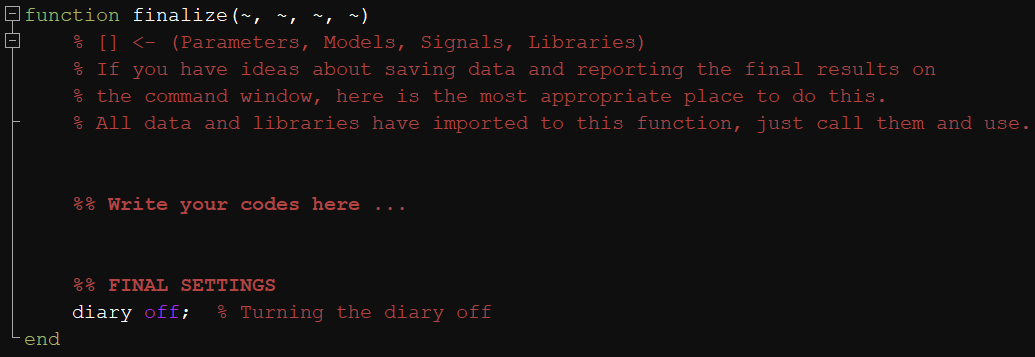
\includegraphics[width=0.95\linewidth,page=1,trim=0 0 0 0,clip=true]{img/matlab/finalize.png}
					\caption{A shot of '\texttt{finalize.m}' function.}
					\label{fig:7}
				}
			\end{figure}
		}
	}
	
	\subsection{Runner classes} {
		\subsubsection{'LTISystem.m'} {
			
		}
		\subsubsection{'nonlinearSystem.m'} {
			
		}
		\subsubsection{'neuronGroup.m'} {
			
		}
		\subsubsection{'estimator.m'} {
			
		}
		\subsubsection{'recursiveLeastSquare.m'} {
			
		}
	}

	\subsection{Observers and detectors} {
		\subsubsection{'scope.m'} {
			
		}
	}
	
	\subsection{Libraries} {
		\subsubsection{'functionLib.m'} {
			
		}
		\subsubsection{'plotLib.m'} {
			
		}
		\subsubsection{'yourLib.m'} {
			
		}
	}
	\subsection{System blocks} {
		
	}
	
}
    }

    \newpage
    \chapter{A Summary of The \LaTeX{} Framework} {
        \newpage

    }

\end{document}